\documentclass[11pt, fullpage,letterpaper]{article}

\usepackage[margin=1in]{geometry}
\usepackage{amsmath}
\usepackage{listings}
\usepackage{graphicx}
\usepackage{hyperref}
\usepackage{amssymb}
\usepackage{placeins}
\usepackage{url}

\hypersetup{
    colorlinks=true,
    linkcolor=blue,
    filecolor=magenta,      
    urlcolor=cyan,
}

\title{Photovoltaic Solar Energy Forecasting}
\author{Roman Amici, Richard Timpson}

\begin{document}

\maketitle

\section{Introduction}

Our project investigated the feasibility of predicting Photovoltaic (PV) energy production in residential solar systems. Residential PV forecasting has typically been limited to apriori models which forecast theoretical average yearly production over the entire lifetime of a system or location. \cite{SAM}. We wanted to assess whether, given weather data, solar irradiance measurements, information about a solar site’s architecture, and hourly measurements of PV production, we could construct a machine learning based model which could accurately forecast energy production at a granular time scale (hour or day) for a specific residential system as an alternative to using the existing apriori models.

A production forecasting system at a granular time scale can be useful for smart home and energy applications on both an individual level and global level. Solar energy is becoming more feasible as an alternative to traditional grid tied power systems, but is still limited by its reliance on power production during a limited time frame. Accurately forecasting the production during that time can enable smart grids and individual PV systems to optimize both power usage and power storage. 

To accomplish this, we built a number of linear regression models. The goals of these models were threefold. The first was simply to establish a baseline model that we could use to compare against other models. The second was to determine, given a set of explanatory features, what class of features were conducive to model performance. Finally, we wanted to determine if the given feature set that we had collected could be used to build a single model that would generalize across multiple different PV energy systems as opposed to a site specific model. 

We believe each of these goals were met although with certain caveats surrounding both data acquisition and modeling. Overall, we see these results as an exploratory baseline which can be used to access further efforts.

\section{Data}

\subsection{Solar PV Energy Production}
The core of our data is centered around energy production data of several different solar photovoltaic panel systems. The data was accessed through a proprietary source so much cannot be said about the production data other than it contains time series data at 15 minute increments for 13 different systems. Some of the systems are built for the rooftop of residential homes and others are for large scale commercial architectures.The range of the data goes back as far as five years for some homes to less than one year for others. Given that the goal of the project is to build a regression model to predict the energy output, the diversity in data lends itself to a higher degree of confidence in the results of a more general model that could be used in a production level software system for any given system with a varying amount of data. Figure \ref{2-1} shows this diversity in the data set.

\begin{figure}[!htb]
    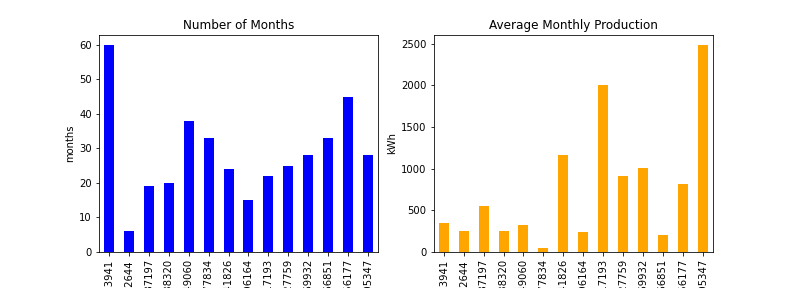
\includegraphics[width=\textwidth]{../plots/regression_report/2-1}
    \caption{Duration (left) and average monthly production (right) for each system. The systems differ significantly. The longest time period is roughly five years whereas the shortest time period is less than a year. There is even more variation in the average monthly production, where the difference in production between the highest and lowest is almost 2000 kWh.}
    \label{2-1} 
\end{figure}

\subsection{Weather Data}
The initial data that was used to build a model was historical weather data pulled for each of the locations of the different systems. Because the data is proprietary no information can be given about the exact locations, but they are all roughly in the southwestern United States. DarkSky \cite{DarkSky} provides an api that gives free access to historical weather data at any location in the United States. We were able to pull the weather data in one hour increments for each location for the entire time period of available production data.

There is one fundamental flaw in this data that we could not solve. For a model whose purpose is to predict the future production of a given system, “historical” weather data does not exist. If weather data were to be used for such a model it would be forecasted weather and not weather that was observed. After many hours spent searching we could never find a data source that provided open access to historical weather \textit{forecasts} – the data that we collected is weather that was actually observed. With the understanding that the data is flawed in this way, we decided to move forward with the data as a proxy for a weather forecast. Although we did not do so, it would have been appropriate to do further research into the difference in accuracy between weather forecasts and observations, as it would in some way inform us about possible errors in our model. Our underlying assumption with the weather data was that it would be close enough to be reliable. 

\FloatBarrier

\subsection{Irradiance Data}

An important factor in modeling almost any photovoltaic energy system is solar irradiance. Solar irradiance is a measure of power per unit area received  from the sun in the form of electromagnetic radiation \cite{nasa}. Solar irradiance can be directly measured on the Earth’s surface or in the atmosphere. It is the most important factor to consider when attempting to forecast the output of a photovoltaic panel system. The National Renewable Energy Laboratory (NREL) maintains a database named the National Solar Radiation Database (NSRDB) which provides historical irradiance measures for any location in the United States \cite{nsrdb}. We pulled from this database to get several measures of solar irradiance for the locations of each of the systems in half hour increments. 

\subsection{System Panel Architecture}

Another dataset that we found useful was the data about the actual panel architecture of the systems for which we had production data. We were able to obtain this data for each system which includes the number of panels and their area, the tilt (measured in degrees and is the angle the panels sit relative to the ground), and azimuth (the direction the panel faces, in most cases directly south). 

\section{Modeling}

In order to investigate the relevant features needed to predict solar output, we built several linear regression models. There are two broad categories of models that we built. One is an individual model for each system, and the other is a generic model that combines data from all systems. For both models we are using ordinary least squares regression. 

\subsection{Data Manipulation and Representation}

The various data sources we gathered provided data in different time intervals. production was at 15 minute, irradiance at half hour, and weather at one hour. We were limited to the longest time interval, so all other data needed to be aggregated to a one hour time interval. Any data points that reported no production value (times during the night), were discarded. The input data was transformed into a vector, $x_i \in R^d$ for each data point serving as the predictor, and a corresponding production value, $y_i$ serving as the target. We use $X^s, Y^s$ to denote the set of all data points $x_i,y_i$ in a particular site, $s \in S$.

\subsection{Feature Representation}

Each training example, $x_i$ can be further broken down into features based on their data source. For our purposes, we will look at $IR_i,W_i,$and $T_i$ which denote Irradiance, Weather and Time respectively. A given train example, $x_i$ will consist of combinations of $IR_i, W_i, T_i$. Irradiance consists of three different measures, Direct Normal Irradiance (DHI), Diffuse Horizontal Irradiance (DHI), and Global Horizontal Irradiance (GHI) \cite{irradiance}. Temporal values include both the time time of day and day of the year. These were then transformed using the nonlinear transformation $1 + sin( \pi t / \tau )$ where $\tau=24$ for hours of the day and $\tau=365$(or $366$) for day of the year. Weather consists of 16 values, some of which are real valued like temperature and precipitation intensity and some which are one-hot encoded categorical variables like precipitation type. See \cite{DarkSky} for the full weather feature set.

\subsection{Cross Validation}

Instead of splitting the data by sampling each hourly training point independently, we made the split such that the set would not be biased toward any particular season or hour of the day. This is more akin to a time-series forecasting model split than a traditional linear model split. We did this by looking at a window of $k$ days at a time and randomly assigned $m / k$ of those days to $X^s_{Train},Y^s_{Train}$ and $(k - m) / k$ days to $X^s_{Test},Y^s_{Test}$. Although this is somewhat unorthodox for a pure linear model, the training and testing set are still drawn from the same distribution and thus we can trust that our evaluations on the test set represent the generalization properties of the model. For our experiments, we chose $k=4$ and $m=3$ leaving 75\% of the days in the training set and 25\% in the test set.

\subsection{Site Specific Models}

The first set of linear models were intended to test the adequacy of specific classes of features for predicting production at a specific site. Thus, we created 13 sets of models, $M^s$ for the 13 separate sites using only $X^s$,$Y^s$. This allowed us to sidestep the ways in which sites might differ from one another and focus only on which variables were useful for predicting solar production. It also served as a baseline which we could compare to transfer learning approaches.
Within each site, we built individual models trained on each combination of feature subsets
\[
    \chi_f^s \in \left\{ IR^s,IR^s + T^s, IR^s + W^s, W^s,W^s + T^s, all \right\}
\] 
where ``all'' denotes $IR^s+W^s+T^s$ and ``$+$'' is used to refer to vector concatenation. 

Within a single site, the performance of each model, $M_f^s$ trained on $\chi_f^s$, can be evaluated to give the relative importance of each feature combination.

\subsection{Transfer Learning}

Our second set of models involved transfer learning. These concerned how well data from other sites could be used to predict production on a different site. We used two different techniques. The first involved building a single integrated model which trained together on the entire training set $X_{Train}=\cup_s X^s_{Train}$. The resulting model, $M_{Int}$ could then be evaluated on each site individually using $Y^s_{Test}$ to obtain $Err(s,M_{Int})$. This allows us to see how well transfer learning does as compared to the original site specific models. 

The second transfer learning approach is an example of “zero shot” learning, where we train on data from all but one cite and then evaluate the model on the held out site. That is, for each site, we train on $X^{s^c}_{Train} = X_{Train} / X^s_{Train}$ and then evaluate the model $M^{s^c}_Z$ on $Y^s_{Test}$ to obtain $Err(s, M^{s^c}_Z)$. Zero-shot learning, therefore, does not train on any data from the site it is evaluated on and is thus the best indicator for how well a model might generalize to brand new sites.

Applying transfer learning without further modification should fail for this data set. This is due to the fact that the magnitude of the output differs based on the size of the site. Thus, it is necessary to add some features which can stand in for the size of the site. In this case we chose to augment $x_i$ with an extra feature $a^s$ which represents the total area of all solar panels in a particular site. This feature is strongly correlated with the total PV production and allows us to side-step this problem.

\section{Results}

The results from the several models we built indicate that the most important data involved in predicting the energy output was solar irradiance and that the model works best when building site specific models. For some of the sites irradiance and time together was sufficient to build close to an optimal model for that site, and for all sites the combination of weather with irradiance seems to be the most important factor in building an accurate model. The transfer learning models were significantly worse than the site specific models.

The metric that we are using to evaluate the model is the root mean squared error (RMSE),which is one of the standard metrics used to evaluate regression models. RMSE simply takes the square root of the mean squared error and provides a more interpretable metric for comparison across models.

\subsection{Site Specific Results}

Because there are a significant number of different models we are comparing we are going to select a few sites that are somewhat representative of the data to graphically show the results of all models. The table in the appendix shows the numerical results of all of the models for all of the different sites. We handpicked four different sites that represent some of the variation in the data – one has data for a long period (site 103941), one has a relatively high monthly average production (717196), and the others are somewhere in between (896164 and 569932). Figure \ref{4-1} shows the RMSE values for each system and for each different site specific model. 

\begin{figure}[!htb]
    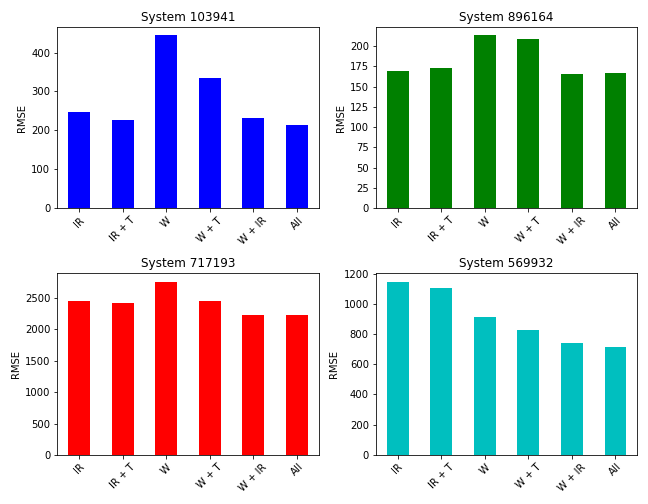
\includegraphics[width=\textwidth]{4-1}
    \caption{RMSE for each feature combination across four different sites. Weather only is typically the worst performing model. Adding irradiance and temporal variables increases the performance to varying degrees, and having all of them together is consistently the best model.}
    \label{4-1}
\end{figure}
To demonstrate a trend amongst all models for all systems, we compare each model to the worst performing model and average those results across all different systems. The worst performing model, on average, is weather only. Here we will define a global model set $$\mathbb{M} = \left\{ M_{IR}, M_{IR+T}, M_{W}, M_{W+T}, M_{W+IR}, M_{all}, M_{Z}, M_{Int} \right\}$$ which represents an aggregate of the different model error results across the different systems. Then 
\[
    \%Diff(M \in \mathbb{M}) = \frac{1}{|S|} \sum_{s \in S} RMSE(M^s_W) - RMSE(M^s)
\]
Figure \ref{4-2} shows the results of this function for all models but weather, which is used for comparison

\begin{figure}[!htb]
    \centering
    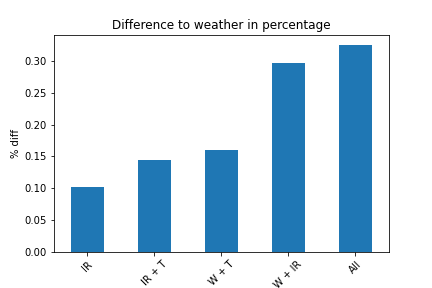
\includegraphics[scale=0.75]{../plots/regression_report/4-2}
    \caption{We see over a 30\% average increase in RMSE when combining all models together. Irradiance alone performs better than weather, and the combination of weather and irradiance almost performs well as well as weather, irradiance, and time together.}
    \label{4-2}
\end{figure}

\subsection{Transfer Learning}

The transfer learning models, as Figure \ref{4-3} shows, perform significantly worse than the site specific models. 
\begin{figure}[!htb]
    \centering
    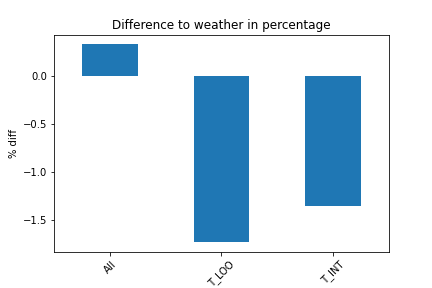
\includegraphics[scale=0.75]{../plots/regression_report/4-3}
    \caption{
        The average of the transfer learning models are close to a factor of 1.5 times worse than the baseline weather only model.
    }
    \label{4-3}
\end{figure}


\FloatBarrier

\section{Discussion}

Our first goal was to build a model which could serve as a baseline for future comparisons. This baseline started with an exploration of weather alone. Adding both irradiance data and temporal variables significantly improves the performance of the model, with irradiance having the larger impact. Irradiance data alone performs better than weather, which indicates that it is the most important feature when forecasting production. We can assume that using all variables together provides a good baseline for further exploration. 

We must, however, be realistic about what this baseline represents. As we have already noted, we used historical weather observations rather than weather forecasts. This thus uses information which would be strictly more accurate than that available in a production system. We should be clear that this represents a sort of “best case scenario” when it comes to using weather variables. We would expect the performance to degrade if we switched to using forecasts instead, since forecasts can obviously be inaccurate. The performance should only degrade past a certain point as it would not be any worse than if we simply removed the weather data from the model entirely. This corresponds to the feature subset case T + IR which still provides competitive performance.

It is hardly surprising, given that solar irradiance is actually a measure of theoretical energy from the sun, that irradiance would be highly predictive of PV output. It is still unclear, however, why there is such a large difference in this impact between the sites (see Figure \ref{4-1}). We hypothesize that it might have to do with the precision of the irradiance measurements at various sites. For irradiance, as for weather, we had to pull data from the external source nearest to our site. This means that the data gathered for each site might differ from the true data at that site (if we could somehow measure it) by varying degrees. If this were the case, then it might explain why irradiance would be less predictive for some sites rather than others. This is a direction we would like to pursue further if time allowed.

Transfer learning, in both the integrated and one-shot cases performed much worse than the individualized models. The most likely possible explanation is that the sites themselves are so different (both in terms of time and in scale) that data from one is not relevant to another. We were only able to integrate one feature from the sites’ configuration (PV area) into the model. There are additional features we could have added such as panel tilt and azimuth but this is difficult to represent because not all panels in a given system are homogenous. This would require a more complex model which could deal with the dynamic sizing of the systems  and was outside of the scope of this project.
    
Another potential avenue we could have explored would have been to try to measure the absolute (as compared to relative) performance of the data. A good place to start would have been to look at the RMSE normalized by the scale of the data although more in depth statistical analysis would be required to quantify this properly.There are also regularization techniques such as lasso and ridge regression that would have been interesting to compare to least-square regression but were not used because of time limitations.
    
The simplest and most important thing that we learned was the importance of irradiance in modeling PV output. Weather turned out to be less impactful than we originally hypothesized and its importance in future models is questionable. We also discovered that a time-series analysis of the data set would be appropriate (perhaps more than regression) for the problem we are modelling but did not have sufficient knowledge to approach the problem from that perspective. How a time-series approach and other modelling choices we mentioned compare to a standard least squares linear regression approach is an open question for future work. What is clear is that now we have a good baseline model and understanding of the problem that we could compare future work to. 


\clearpage

\bibliography{references}
\bibliographystyle{plain}

\section*{Appendix}

\subsection*{Data Table}
Table of RSME for each feature combination (rounded to the nearest whole number).
\begin{center}
    \begin{tabular}{|c|c|c|c|c|c|c|c|c|}
        \hline
        Site ID & $M_{IR}$ & $M_{IR + T}$ & $M_{W}$ & $M_{W + T}$ & $M_{W + IR}$ & $M_{all}$ & $M_{Z}$ & $M_{Int}$ \\
        \hline
        103941 & 246&225&443&333&230&214&1408&962 \\
        \hline
        787197&458&441&676&493&420&414&1139&1051 \\
        \hline
        238320&406&400&215&194&180&179&1216&1046 \\
        \hline
        349060&195&195&366&277&173&172&1063&906 \\
        \hline
        477834&185&182&180&165&146&141&1084&1027 \\
        \hline
        641826&1415&1356&1400&1340&1129&1074&1892&1740 \\
        \hline
        896164&169&173&213&209&165&166&977&936 \\
        \hline
        717193&2452&2423&2755&2454&2235&2228&3167&3074 \\
        \hline
        627759&661&562&1158&830&604&553&987&943\\
        \hline
        569932&1144&1107&912&824&742&714&1280&1185 \\
        \hline
        466851&391&388&387&351&325&314&803&777 \\
        \hline
        256177&1250&1007&1464&1117&1103&967&4347&2328 \\
        \hline
        505347&2176&1857&3596&2653&2004&1799&6092&5290 \\
        \hline

    \end{tabular}
\end{center}

\subsection*{Division of the Work}

\begin{center}
\begin{tabular}{|l|l|}
    \hline
    Task & Who?\\
    \hline
    Collect Solar Production Data & Richard \\
    \hline
    Collect Weather Data & Roman \\
    \hline
    Collect Irradiance Data & Richard \\
    \hline
    Data Cleaning & Roman \\
    \hline
    Initial Linear Model & Richard \\
    \hline
    Site Specific Models & Roman \\
    \hline
    Transfer Learning Models & Roman \\
    \hline
    Visualization and Data Analysis & Richard \\
    \hline
\end{tabular}
\end{center}

\end{document}